% Introduction. Numbers: results/complementarity/{retrieval_vs_selection,private_batch_profile}.md,
% results/client_encoder_plain/summary.md, results/heldout_rerun/summary.md, results/complementarity/floor_baselines.md.
\section{Introduction}
\label{sec:intro}

\begin{figure*}[t]
\centering
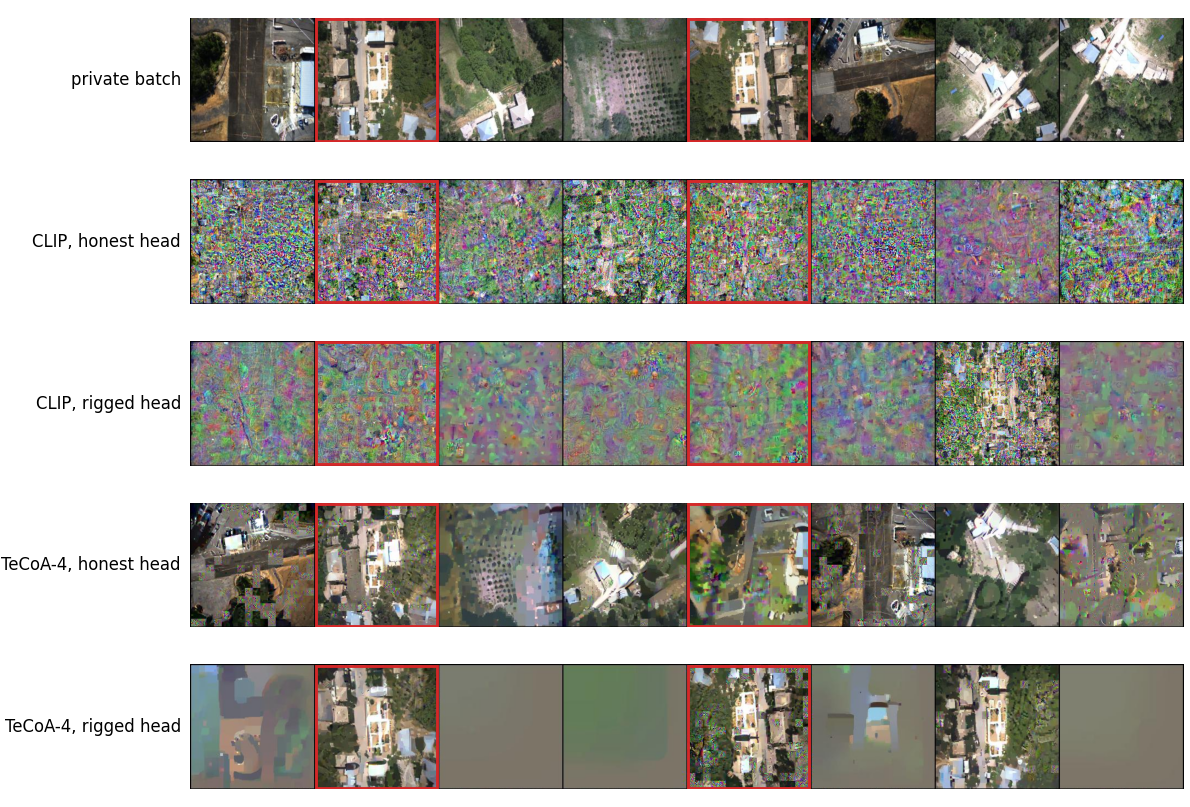
\includegraphics[width=\textwidth]{fig/recon_uav_backbone}
\caption{\textbf{Selection and invertibility are separate factors.} Top row: a client's private batch of eight drone frames, two of which (red) show the rooftop solar panels the attacker asked for. Below: HF-GradInv reconstructions from one shared gradient when the client model is built on vanilla CLIP or on the adversarially fine-tuned TeCoA-4 encoder, each under an honest classifier head and under the head \geminio rigs for the query. The honest head on TeCoA-4 reconstructs the whole batch moderately; the rigged head on TeCoA-4 reconstructs the two targets sharply and sacrifices the rest; on vanilla CLIP neither head recovers anything. Same seed throughout.}
\label{fig:teaser}
\end{figure*}

Federated learning (FL) is sold to hospitals and to operators of camera-equipped drones as a way to train a shared model without ever pooling the images.
Gradient inversion attacks undercut that promise: an honest-but-curious server can optimize dummy inputs until their gradients match the ones a client sent and so recover the client's training images~\cite{dlg2019,ig2020,gradinversion2021}.
A \emph{malicious} server can do better, because it also chooses the model the clients compute gradients on~\cite{robbing2022,fishing2023,garov2024seer}.
\geminio~\cite{geminio2024} is the most targeted attack in this family.
The server writes down what it wants in natural language (``any chest X-ray showing pneumonia''), scores a pool of unlabeled auxiliary images against that query with a vision-language model (VLM), and trains the classifier head it distributes so that images the VLM ranks highly incur a large loss.
When an honest client trains on a private batch, the query-matched images dominate the shared gradient, and an off-the-shelf reconstruction algorithm recovers them.

This paper asks a plain question about that attack: what decides whether it recovers the images it was asked for?
Two ingredients are in play, and prior work has studied them separately.
Malicious-server attacks concentrate the gradient on a few samples~\cite{fishing2023,robbing2022}; adversarially trained models leak more under gradient inversion because their features are easier to invert~\cite{zhang2022privacyat,mejia2019robustorprivate,torp2026nonrobust}.
Adversarially fine-tuned CLIP encoders (TeCoA~\cite{tecoa2023}, FARE~\cite{fare2024}, Sim-CLIP~\cite{simclip2024}) are now the standard way to harden vision-language models, and they can enter the \geminio pipeline in two places: as the attacker's guide, and as the backbone of the client model whose gradient is inverted.
We treat the attack as the product of two factors, \emph{selection}, the share of the client's gradient that the rigged head places on the query-matched images, and \emph{invertibility}, how well the client backbone's features reconstruct, and we measure both directly rather than inferring them from reconstruction quality.

\paragraph{Findings.}
We evaluate \geminio on chest X-rays (ChestMNIST), colorectal histology (PathMNIST) and aerial drone imagery (UAVScenes), with eight guiding VLMs, a ResNet-18 client and ten ViT-L client backbones, three reconstruction algorithms and three seeds per condition, on held-out private batches the rigged heads never saw.
\begin{enumerate}
\itemsep0pt
\item \textbf{Selection tracks the guide's retrieval.} For each of 25 attacker configurations we compute the two target images' share of the summed per-example last-layer weight-gradient norms on the private batch. It is rank-correlated with how well the guide ranks the target class on the auxiliary set (Spearman $\rho=0.67$ over 25 heads; $p=.001$ under a dataset-stratified permutation null). Where the guide ranks the class well the rigged head puts more of that norm on the targets than an honest head does, and on ChestMNIST, where no guide ranks \pneu above 0.64 AUROC, it puts less; no configuration in the project reconstructs a chest X-ray more closely than eight images drawn at random from the dataset (\cref{sec:selection}).
\item \textbf{Robust client backbones reveal what the head selects.} With the query-matched images selected, adversarially fine-tuned ViT-L backbones leak them more than vanilla CLIP (6 of 6, ordered by robustness level) and more selectively; an honest head on the same encoders gives no selectivity, and rigging the head for a different class moves the selectivity to that class. \TODO{comparators: LAION-2B CLIP, DINOv2, supervised IN-21k ViT-L; queue running} (\cref{sec:backbone}).
\item \textbf{Robust guides change reconstruction quality, not selection.} As the attacker's guide, every robust CLIP makes the ChestMNIST attack reconstruct the batch better than vanilla CLIP (18 of 18 seed pairs), yet none of their heads places more than the uniform share of the gradient on the \pneu images. \TODO{PathMNIST guide table, queue running} (\cref{sec:guide}).
\item \textbf{Defense and failure cases.} Noisy, clipped per-update aggregation (\nbfu) removes the drone-imagery reconstruction that the Inverting Gradients attack achieves and weakens \geminio across a 24-query language sweep; clipping alone does nothing. Indirect and terse queries break the attack, misspelled, translated and negated queries do not, and retrieval failure is its dominant failure mode (\cref{sec:failure,sec:defense}).
\end{enumerate}
Along the way we correct two practices from the \geminio evaluation protocol that hid these results: the attack-F1 metric, which scores pure-noise reconstructions near 1.0, and the absence of a reference for what an uninformative reconstruction scores, which we supply with random draws from the dataset scored through the same matching code.
